\section{Propagator}
\label{section:propagator}

We may write the quadratic part of the Lagrangian \autoref{L2} as \footnote{Summation over isospin index ($a,b,c$) will be explicit in this section.}
\begin{align}
    \label{quadratic lagrangian}
    \Ell_2^{(2)}
    =
    \frac{1}{2} \sum_a \partial_\mu \pi_a \partial^\mu \pi_a
    + \frac{1}{2} m_{12} (\pi_1 \partial_0 \pi_2 - \pi_2 \partial_0 \pi_1)
    - \frac{1}{2} \sum_a m_a^2 \pi_a^2,
\end{align}
where
\begin{align}
    \label{m1}
    m_1^2 &= \bar m^2 \cos{\alpha} - \mu_I^2 \cos{2\alpha}, \\
    \label{m2}
    m_2^2 &= \bar m^2 \cos{\alpha} - \mu_I^2 \cos^2{\alpha}, \\
    \label{m3}
    m_3^2 &= \bar m^2 \cos{\alpha} + \mu_I^2 \sin^2{\alpha}, \\
    \label{m12}
    m_{12} &= 2 \mu_I \cos{\alpha}.
\end{align}
The components of the Euler-Lagrange equations of this field are
\begin{equation*}
    \pdv{\Ell}{\pi_a} = 
    \frac{1}{2} m_{12} (\delta_{a1} \partial_0 \pi_2 - \delta_{a2}\partial_0 \pi_1) 
    - m^2_{a} \pi_a, \quad
    \pdv{\Ell}{(\partial_\mu \pi_a)} = 
    \partial^\mu \pi_a - \frac{1}{2} m_{12} \delta^\mu_0 (\delta_{a1}\pi_2  - \delta_{a2}\pi_1).
\end{equation*}
This gives the equation of motion for the field
\begin{equation}
    \partial^\mu \partial_\mu \pi_a + m_a^2 \pi_a
    =  m_{12}(\delta_{a1} \partial_0 \pi_2  - \delta_{a2} \partial_0 \pi_1).
\end{equation}
The propagator of the pion field is defined by
\begin{equation}
    \left[
        \delta_{ab}(\partial^\mu\partial_\mu + m^2_a)
        -  m_{12}(\delta_{a1} \delta_{b2} - \delta_{a2}\delta_{b1}) \partial_0
    \right] 
    D_{bc}(x, x') 
    = -i \delta(x - x') \delta_{ac}.
\end{equation}
The momentum space propagator, as defined in the \autoref{Conventions and notation}, fulfills (MOTSATT FORTEGN FRA FRI ENERGI; FIKS!!!)
\begin{equation*}
    -\left[
        \delta_{ab}(p^2 - m_a^2)
        +  i p_0 m_{12}(\delta_{a1} \delta_{b2} - \delta_{a2}\delta_{b1}) 
    \right] 
     D_{bc}(p) 
    := D^{-1}_{ab}  D_{bc}(p) = -i \delta_{ac},
\end{equation*}
where
\begin{equation*}
    D^{-1} = -
    \begin{pmatrix}
        p^2 - m^2_1             & i p_0 m_{12}     & 0             \\
        - i p_0 m_{12}            & p^2 - m^2_2       & 0             \\
        0                       & 0                 & p^2 - m^2_3
    \end{pmatrix}.
\end{equation*}
The spectrum of the particles is given by solving $\det(D^{-1}) = 0$ for $p^0$. With $p = (p_0, \vv p)$ as the four momentum, this gives
\begin{align*}
    \det(D^{-1}) & = D^{-1}_{33} \left(D^{-1}_{11} D^{-1}_{22} + (D^{-1}_{12})^2\right)
    = - \left(p^2 - m^2_3\right)
    \left[
        \left(p^2 - m^2_1\right)
        \left(p^2 - m^2_2\right)
        - p_0^2 m_{12}^2
    \right] = 0,
\end{align*}
This equation has the solutions
\begin{align}
    \label{dispresion relation pi 0}
    E_0^2 &= |\vv p|^2 + m_3^2, \\
    \label{dispresion relation pi pm}
    E_\pm^2
    & = |\vv p|^2 +
    \frac{1}{2}
    \left(
        m_1^2 + m_2^2 + m_{12}^2 
    \right)
    \pm 
    \frac{1}{2}
    \sqrt{
        4|\vv p|^2m_{12}^2 
        +
        \left(
            m_1^2 + m_2^2 + m_{12}^2
        \right)^2
        - 4 m_1^2 m_2^2
    }.
\end{align}
These are the energies of three particles $\pi_0$, $\pi_+$ and $\pi_-$.
$\pi_0$ is $\pi_3$, while $\pi_\pm$ are linear combinations of $\pi_1$ and $\pi_2$.
The (tree-level) masses of these particles are found by setting $\vv p = 0$, i.e. the rest-frame energy, and are
\begin{align}
    m_0^2 &= m_3^2, \\
    m_\pm^2
    & =  \frac{1}{2}
    \left[
        m_1^2 + m_2^2 + m_{12}^2 
    \right]
    \pm \frac{1}{2}
    \sqrt{
        \left(
            m_1^2 + m_2^2 + m_{12}^2
        \right)^2
        - 4 m_1^2 m_2^2
    }.
\end{align}
\autoref{fig:masses} shows the masses as functions of $\mu_I$.

\begin{figure}[h]
    \centering
    % \vspace{-2cm}
    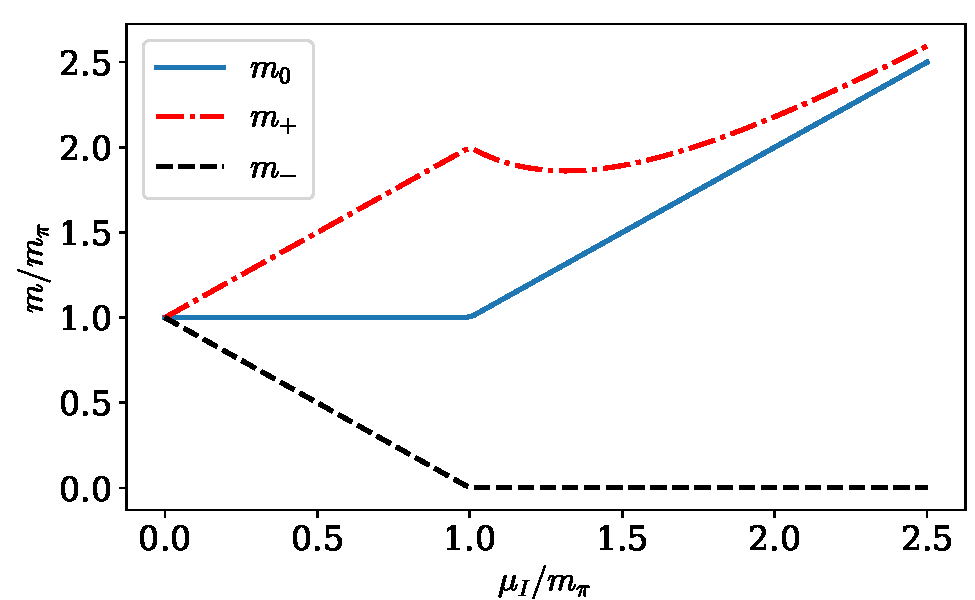
\includegraphics[width=0.7\textwidth]{figurer/numerics/masses.pdf}
    \caption{The masses of the three particles as functions of isosopin chemical potential.}
    \label{fig:masses}
\end{figure}

With these energies we can write the determinant of the inverse propagator as
\begin{equation}
    \det(D^{-1}) = - (p_0^2 - E_0^2) (p_0^2 - E_+^2) (p_0^2 - E_-^2).
\end{equation}
The propagator may then be obtained as described in \autoref{Conventions and notation},
\begin{align}
    \notag
    D & = i (D^{-1})^{-1} = \frac{i}{\det(D^{-1})}
    \begin{pmatrix}
        D^{-1}_{22} D^{-1}_{33}   & D^{-1}_{12}D^{-1}_{33}  & 0 \\
        -D^{-1}_{12}D^{-1}_{33}   & D^{-1}_{11}D^{-1}_{33}  & 0 \\
        0               & 0             & D^{-1}_{11}D^{-1}_{22} + (D^{-1}_{12})^2
    \end{pmatrix} \\
    \label{free pion propagator}
    & = i
    \begin{pmatrix}
        \frac{
            p^2 - m_2^2
        }
        {
            (p_0^2 - E_+^2)(p_0^2 - E_-^2)
        } 
        & \frac{
            - ip_0m_{12}
        }
        {
            (p_0^2 - E_+^2)(p_0^2 - E_-^2)
        } & 0 \\
        \frac{
            ip_0m_{12}
        }
        {
            (p_0^2 - E_+^2)(p_0^2 - E_-^2)
        }
        & \frac{
            p^2 - m_1^2
        }
        {
            (p_0^2 - E_+^2)(p_0^2 - E_-^2)
        } & 0 \\
        0 & 0 & 
        \frac{1}{p_0^2 - E_0^2}
    \end{pmatrix}.
\end{align}
